% Copyright 2004 by Till Tantau <tantau@users.sourceforge.net>.
%
% In principle, this file can be redistributed and/or modified under
% the terms of the GNU Public License, version 2.
%
% However, this file is supposed to be a template to be modified
% for your own needs. For this reason, if you use this file as a
% template and not specifically distribute it as part of a another
% package/program, I grant the extra permission to freely copy and
% modify this file as you see fit and even to delete this copyright
% notice. 

\documentclass{beamer}
% \usepackage{subcaption}
% There are many different themes available for Beamer. A comprehensive
% list with examples is given here:
% http://deic.uab.es/~iblanes/beamer_gallery/index_by_theme.html
% You can uncomment the themes below if you would like to use a different
% one:
% \usetheme{AnnArbor}
% \usetheme{Antibes}
% \usetheme{Bergen}
% \usetheme{Berkeley}
% \usetheme{Berlin}
% \usetheme{Boadilla}
% \usetheme{boxes}
% \usetheme{CambridgeUS}
% \usetheme{Copenhagen}
% \usetheme{Darmstadt}
% \usetheme{default}
% \usetheme{Frankfurt}
% \usetheme{Goettingen}
% \usetheme{Hannover}
% \usetheme{Ilmenau}
% \usetheme{JuanLesPins}
% \usetheme{Luebeck}
\usetheme{Madrid}
% \usetheme{Malmoe}
% \usetheme{Marburg}
% \usetheme{Montpellier}
% \usetheme{PaloAlto}
% \usetheme{Pittsburgh}
% \usetheme{Rochester}
% \usetheme{Singapore}
% \usetheme{Szeged}
% \usetheme{Warsaw}

\title[COP 290]{Space Invaders}

\subtitle{COP290: Assignment 3}

\author[Faran \and Kabir \and Kartikeya \and Prateek]{Faran Ahmad \and Kabir Chhabra \and Kartikeya Gupta \and Prateek Verma \\
  2013CS10220 \and 2013CS50287 \and 2013CS10231 \and 2013CS10246}

\institute[IITD] % (optional, but mostly needed)
{
  Department of Computer Science and Engineering\\
  IIT Delhi
}

\date{March 16, 2015}
\subject{Design Practices}

\AtBeginSubsection[]
{
  % \begin{frame}<beamer>{Outline}
  %   \tableofcontents[currentsection,currentsubsection]
  % \end{frame}
}

\begin{document}

\begin{frame}
  \titlepage
\end{frame}

\begin{frame}{Objectives}{}
	Design a game which is :
	\begin{itemize}
		\item Multi-player on-line without a central server.
		\item Has a artificial intelligence component.
		\item Is an action game and not a simple board game.
	\end{itemize}
\end{frame}

\begin{frame}{Our choice}{Space Invaders}
    \begin{figure}[ht!]
      \centering
          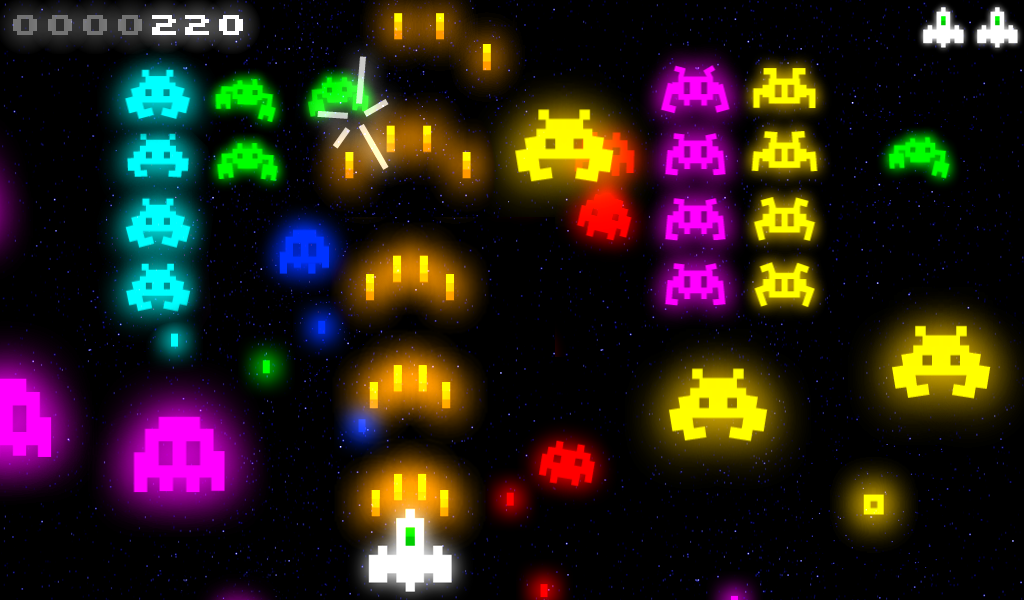
\includegraphics[width=1.0\linewidth]{gameplay.png}
    \end{figure}
\end{frame}


\begin{frame}{Space Invaders}{Basic Game-play}
  \begin{itemize}
  	\item The player will control a space ship and shoot down aliens.
  	\item The player will be allowed to move in the 2D plane and change its orientation in that plane 
  	\item The aliens will shoot bullets at the players ship.
  	\item On getting hit by bullets the player will lose 1 life.
  	\item On destroying a large number of aliens, the player will get bonus lives.
  \end{itemize}
\end{frame}

\begin{frame}{Space Invaders}{Multi-player}
	\begin{block}{Co-op Mode}
	\begin{itemize}
		\item In co-op mode, the different players will team up to fight the aliens.
		\item The points scored by each will be combined together.
	\end{itemize}
	\end{block}
	\begin{block}{Competitive mode}
	\begin{itemize}
		\item Players will be put up against each other, every player for himself. 
		\item Each player has its own score which will be increased on hitting the other players.
	\end{itemize}  
	\end{block}
\end{frame}

\begin{frame}{Space Invaders}{Scoring Scheme}
	\begin{block}{Lives}
		\begin{itemize}
			\item Each player will be given 3 lives.
			\item On getting hit by an alien bullet or colliding with an alien, a life will be lost.
			\item After killing 10 aliens in a row without any waste shot, a life will be awarded.
		\end{itemize}
	\end{block}
	
	\begin{block}{Scoring}
		\begin{itemize}
			\item On killing an alien a point would be avoided.
			\item On killing more and more aliens in a row, a multiplying factor associated with points would increase.
		\end{itemize}
	\end{block}
\end{frame}


\begin{frame}{Network Design}{}
	\begin{block}{Basic Design}
		\begin{itemize}
			\item Our application will use UDP (User Datagram Protocol) to communicate between various players.
			\item Since our multi-player is real time, we need fast transfer of data.
			\item Even if some of the packets are lost due to unreliability of UDP, it won't affect much. Things change so fast (i.e. player movement) in the game that it doesn't make sense to resend a lost packet as it will contain old information.
		\end{itemize}
	\end{block}
\end{frame}

\begin{frame}{Network Design}{}	
	\begin{block}{Idea}
		\begin{itemize}
			\item Each player will have two basic threads.
			\item One thread for receiving data from other players.
			\item Second thread for sending data to other players.
		\end{itemize}
	\end{block}

	\begin{block}{Exchanging data}
		\begin{itemize}
			\item We will send data from one player to all the other players as soon as a frame is rendered
			\item This means that we will send almost 30-60 messages every second and hence UDP is used.
		\end{itemize}
	\end{block}
\end{frame}

\begin{frame}{Network Design}{Network Outages}
	\begin{block}{Connection lost}
		\begin{itemize}
			\item If a player disconnects, AI (same level) will take over the ship.
			\item Once the player reconnects, he will automatically gain control of his lost ship.
		\end{itemize}
	\end{block}	
	\begin{block}{Concept of ``server''}
		\begin{itemize}
			\item When a game is setup, a randomly chosen player will act as a ``temporary server''.
			\item This player will act as the AI of the game and will send messages to all the other players accordingly.
			\item If a player other than this one disconnects, no change is required.
			\item If this player disconnects, another active player will be chosen to act as the ``temporary server''.
		\end{itemize}
	\end{block}
\end{frame}

\begin{frame}{Artificial Intelligence}{Overview}
  The working of the enemy/opponent will be based on the concept of finite state machines where the enemy/ opponent will transition between particular states based on the situation. Different states define different modes of operation which include attacking, dodging or fleeing.
\end{frame}

\begin{frame}{Artificial Intelligence}{}
	\begin{block}{Enemy}
  			Difficulty Level : Three Difficulty levels: easy medium and hard. \\
			Enemy: Speed of enemy and frequency of bullets fired will be a function of difficulty.
 	\end{block}
	\begin{block}{Opponent} 
  			Accuracy of the opponent, frequency of bullets fired, and dodging ability of the opponent will be a function of difficulty.
	\end{block}
	\begin{block}{Incorporation}
		For games with simple entities, Entity pull systems work best where entities call on the AI system when they update themselves.
	\end{block}
\end{frame}

\begin{frame}{Time Line}{}
	  \begin{center}
    \begin{tabular}{ | l | p{9cm} |}
    \hline
    Date &  Summary \\ \hline
    31 April & Graphics of individual components like aliens, ships etc. Basic network communication.\\ \hline
    07 May & AI of the ships. Dealing with network outages.\\ \hline
    14 May & AI of the aliens. Integrating AI with main game. Testing the network component. \\ \hline
    21 May & Integration of all components together. \\ \hline
    24 May & Rigorous testing and submission. \\ 
    \hline
    \end{tabular}
\end{center}
\end{frame}

\begin{frame}{End}
	\vfill
	\begin{center}
		\Huge{Thank You}
	\end{center}
	\vfill
\end{frame}

\end{document}